\documentclass[xcolor=dvipsnames]{beamer} 

%\includeonlyframes{titlepage,background,algebras,algexamples,lattices,distributivity,%
%eqlat,conglat2,congruences,conglat1,groupcong,subglat,hasseexample,info,flrp}
%\includeonlyframes{eqlatex,concrete,galois,closure}
%\includeonlyframes{info,closure,results}
%\includeonlyframes{results,results2,results3,results4,results5,summary}

%\usepackage{enumerate,amsmath,amssymb,fancyhdr,mathrsfs,amsthm}
\usepackage{mathrsfs,textcomp}
%\documentclass[draft]{beamer} 
%\documentclass{beamer} 
\setbeamertemplate{navigation symbols}{}
\usepackage{verbatim}
\usepackage[mathcal]{euscript}

\usecolortheme[named=OliveGreen]{structure} 
\setbeamertemplate{items}[ball] 
\setbeamertemplate{blocks}[rounded][shadow=true] 
% - Talk at a conference/colloquium.
% - Talk length is about 20min.
% - Style is ornate.

% This changes the color of alerted text to blue:
\definecolor{MyDarkBlue}{rgb}{0.2,0.2,0.7}
\setbeamercolor{alerted text}{fg=blue}
\newcommand{\emphcyan}[1]{\textcolor{MyDarkBlue}{\textbf{#1}}}
%\renewcommand{\alert}[1]{\textcolor{MyDarkBlue}{\emph{#1}}}
% (default is red, but my slides are green and I don't like red and green together)


\newcommand{\Hawaii}{Hawai\kern.05em`\kern.05em\relax i}
\newcommand{\Manoa}{M\=anoa}
\newcommand{\cd}{\ensuremath{\otimes}}
\newcommand{\con}[1]{\ensuremath{\langle #1 \rangle}}
\newcommand{\ii}[1]{{\it #1}}
\newcommand{\power}[1]{\ensuremath{\mathscr{P}(#1)}}
\newcommand{\scrA}{\ensuremath{\mathscr{A}}}
\newcommand{\bM}{\ensuremath{\mathbf{M}}}
\newcommand{\Mn}{\ensuremath{\mathbf{M}_n}}
\newcommand{\bF}{\ensuremath{\mathbf{F}}}
\newcommand{\bE}{\ensuremath{\mathbf{E}}}
\newcommand{\bR}{\ensuremath{\mathbf{R}}}
\newcommand{\bA}{\ensuremath{\mathbf{A}}}
\newcommand{\bG}{\ensuremath{\mathbf{G}}}
\newcommand{\bH}{\ensuremath{\mathbf{H}}}
\newcommand{\bK}{\ensuremath{\mathbf{K}}}
\newcommand{\bL}{\ensuremath{\mathbf{L}}}
\newcommand{\bB}{\ensuremath{\mathbf{B}}}
\newcommand{\svert}{\ensuremath{\; \vert \; }}

\newcommand{\sE}{\ensuremath{\mathcal{E}}}
\newcommand{\sH}{\ensuremath{\mathcal{H}}}
\newcommand{\sS}{\ensuremath{\mathcal{S}}}
\newcommand{\sL}{\ensuremath{\mathcal{L}}}
\newcommand{\bN}{\ensuremath{\mathbf{N}}}
\newcommand{\bX}{\ensuremath{\mathbf{X}}}


\newcommand{\sA}{\ensuremath{\mathcal{A}}}
\newcommand{\sB}{\ensuremath{\mathcal{B}}}
\newcommand{\sC}{\ensuremath{\mathcal{C}}}
\newcommand{\SSS}{\text{\emphslb{S}}}
\newcommand{\id}{\mbox{id}}
\newcommand{\Hom}{\mbox{Hom}}
\newcommand{\Con}{\mbox{Con}}
\newcommand{\bCon}{\ensuremath{\mathbf{Con}}}
\newcommand{\Stab}{\mbox{Stab}}
\newcommand{\bStab}{\ensuremath{\mathbf{Stab}}}
\newcommand{\Sub}{\mbox{Sub}}
\newcommand{\bSub}{\ensuremath{\mathbf{Sub}}}
\newcommand{\CSub}[1]{\ensuremath{\mathbf{CSub}[#1]}}
\newcommand{\X}{\ensuremath{\mathbf{X}}}
\newcommand{\csub}{\ensuremath{\mbox{CSub}}}
\newcommand{\image}{\mbox{im}}
\newcommand{\Eq}{\mbox{Eq}}
\newcommand{\bEq}{\ensuremath{\mathbf{Eq}}}
\newcommand{\bEqX}{\ensuremath{\mathbf{Eq}(X)}}
\newcommand{\idemdec}{\ensuremath{\mbox{Idemdec}(X)}}
\newcommand{\EqX}{\ensuremath{\mbox{Eq}(X)}}
\newcommand{\upalpha}{\ensuremath{\alpha^{\uparrow}}}
\newcommand{\downalpha}{\ensuremath{\alpha^{\downarrow}}}
\newcommand{\upbeta}{\ensuremath{\beta^{\uparrow}}}
\newcommand{\downbeta}{\ensuremath{\beta^{\downarrow}}}
\newcommand{\meet}{\ensuremath{\wedge}}
\newcommand{\join}{\ensuremath{\vee}}
\newcommand{\Meet}{\ensuremath{\bigwedge}}
\renewcommand{\Join}{\ensuremath{\bigvee}}

%%% Freese Macros %%%
%%%=================Emphasizing with bold=================

%\DeclareRobustCommand\emb
%        {\@nomath\emb \ifdim \fontdimen\@ne\font >\z@
%                       \upshape \else \bfseries \fi}
%
%
%\DeclareTextFontCommand{\emphb}{\emb}

%\DeclareRobustCommand\emslb
%        {\@nomath\emb \ifdim \fontdimen\@ne\font >\z@
%                       \bfseries\slshape \else \bfseries\slshape \fi}
\DeclareRobustCommand\emslb{\bfseries\slshape}
\DeclareTextFontCommand{\emphslb}{\emslb}
\newcommand{\alg}[1]{\mathbf{#1}}
\newcommand{\HH}{\text{\emphslb{H}}}
\renewcommand{\SS}{\text{\emphslb{S}}}
\newcommand{\PP}{\text{\emphslb{P}}}
\newcommand{\II}{\text{\emphslb{I}}}
\newcommand{\VV}{\text{\emphslb{V}}}
\newcommand{\vr}{\VV}
\newcommand{\Ps}{\PP_{\text{\emphslb{s}}}}
\newcommand{\Si}{\SS_{\text{\emphslb{i}}}}
\renewcommand{\Pr}{\PP_{\text{\emphslb{r}}}}
\newcommand{\Pu}{\PP_{\text{\emphslb{u}}}}
\newcommand{\Se}{\SS^{\prec}}
\newcommand{\urt}{\sqrt[\text{\emphslb{u}}]}
\newcommand{\la}{\langle}	     %% left angle for order sequences <a,b>
\newcommand{\ra}{\rangle}	     %% right angle

 \mode<presentation>
 {
%   \setbeamertemplate{background canvas}[vertical shading][bottom=green!10,top=gray!10]
%   \usetheme{Warsaw}
   \usetheme{Madrid}
   % or ...
   %\setbeamercovered{transparent}
   % or whatever (possibly just delete it)
 }

\usepackage[english]{babel}
\usepackage[latin1]{inputenc}
\usepackage{times}
\usepackage[T1]{fontenc}
% Or whatever. Note that the encoding and the font should match. If T1
% does not look nice, try deleting the line with the fontenc.

\title[Finite Lattice Representation Problem] % (optional, will appear at bottom of each slide)
{The Finite Lattice Representation Problem}
%\subtitle{intervals in subgroup lattices and \\ the dawn of tame congruence theory}


\author[W.J.~DeMeo]{William J.~DeMeo}
%\institute[University of \Hawaii]%
%{University of \Hawaii\ at \Manoa}
\institute[\Hawaii]{University of \Hawaii}

\date[KMS-AMS 2009]% (optional, should be abbreviation of conference name)
{KMS-AMS Joint Meeting\\
December 18, 2009}
%\date[Honolulu 2009]{Math 613: Group Theory\\ November 2009}

\subject{Universal Algebra; Lattice Theory.}% (optional) inserted into PDF info catalog.

% TOC pops up at the beginning of each subsection:
% \AtBeginSubsection[]
% {
%   \begin{frame}<beamer>
%     \frametitle{Outline}
%     \tableofcontents[currentsection,currentsubsection]
%   \end{frame}
% }

% If you wish to uncover everything in a step-wise fashion, uncomment
% the following command: 
%\beamerdefaultoverlayspecification{<+->}

\begin{document}
\thicklines

\frame[label=titlepage]{
  \titlepage
}

% \begin{frame}
%   \frametitle{Outline}
%   \tableofcontents
%   % You might wish to add the option [pausesections]
% \end{frame}

%\section{Introduction}

 
%% 2.
\frame[label=background]{
  \frametitle{Background}
    \begin{theorem}[{\small Gr\"{a}tzer-Schmidt, 1963}]
      Every algebraic lattice is isomorphic to
      the congruence lattice of\\ an algebra.
    \end{theorem}
  \uncover<2->{%
    In particular, this shows there is no lattice-theoretic condition
    stronger than algebraicity satisfied by all congruence lattices.
  }
  \uncover<3->{%
    \begin{block}{What if the lattice is finite?}{}
    }
    \uncover<4->{%
      \underline{Problem}: Given a finite lattice \bL, does there exist a
      \emph{finite}
      \phantom{\underline{Problem}: }algebra \bA\ such that $\bCon\bA \cong \bL$?
    }
    \uncover<5->{%
      \begin{columns}
        \column{0mm}
        \column{108mm}
        \begin{itemize}
        \item[\underline{status}:] open
        \item[\underline{age}:] 45+ years
          % \item[\underline{difficulty}:] probably hard
        \end{itemize}
      \end{columns}
    \end{block}
  }
}% end frame: background


%%\subsection{Universal Algebra}
%\subsection{algebras and their congruences}
%% 2.
\frame[label=algebras]{
  \frametitle{What is an algebra?}
%  \framesubtitle{Subtitles are optional.}
  % - A title should summarize the slide in an understandable fashion
  %   for anyone how does not follow everything on the slide itself.

  \begin{definition}[algebra]
    An \alert{algebra} $\bA$ is an ordered pair $\bA = \langle A, F\rangle$ where
    \begin{itemize}
    \item<1->[] $A$ is a nonempty set, called the \emph{universe} of \bA
    \item<1->[] $F$ is a family of finitary operations acting on $\bA$
    \end{itemize}
    \uncover<2->{An algebra $\langle A, F \rangle$ is \alert{finite} if $|A|$ is finite.}
  \end{definition}

  \begin{itemize}
    \item<3->
      Examples: semigroups, groups, rings, modules, lattices, $*$-algebras
      (with a vector space reduct, ring reduct, and unary $^*$)
%      quasigroups, Boolean algebras, etc.
    \item<4->
      A \emphcyan{variety} $\mathcal K$ of algebras is a class of
      (similar) algebras defined by equations. 
      They are closed under homomorphic
      images, subalgebras and direct products, and in fact
      \[
      \VV(\mathcal K) = \HH\SSS\PP(\mathcal K)
      \]
      is the variety generated by a class $\mathcal K$ of algebras.
%     \item<5->
%       Varieties are closed under homomorphic images, subalgebras and
%       direct products. In symbols,
%       \[
%       \HH(\mathcal K) = \mathcal K, \quad
%       \SSS(\mathcal K) = \mathcal K, \quad
%       \PP(\mathcal K) = \mathcal K
%       \]
%     \item<5-> The variety generated by a class $\mathcal K$ of algebras
%       consists of all homomorphic images, subalgebras and
%        direct products:
%       \[
%       \VV(\mathcal K) = \HH\SSS\PP(\mathcal K)
%       \]
  \end{itemize}

}

% is \emph{finite} if $|A|$ is finite and \emph{trivial} if $|A| = 1$.
% Given two algebras $\bA$ and $\bB$, we say that $\bB$ is a 
% \emph{reduct} of $\bA$ if both algebras have the same universe and $\bA$
% can be obtained from $\bB$ by simply adding more operations.
% %that is, roughly speaking, $B = A$ and $F^{\bB}\subseteq F^{\bA}$.
% % =\langle B, F^\bB \rangle$ % =\langle A, F^A \rangle$,


\frame[label=algexamples]{
  \frametitle{Examples}
  \begin{itemize}
  \item<1->  A \alert{group} is an algebra $\bG = \langle G, \cdot, ^{-1}, 1\rangle$ 
    with binary, unary, and nullary operations satisfying, $\forall x, y, z\in G$,
    \begin{itemize}
    \item[G1:] $x\cdot (y\cdot z) \approx (x\cdot y)\cdot z$
    \item[G2:] $x\cdot 1\approx 1\cdot x \approx x$
    \item[G3:] $x\cdot x^{-1} \approx x^{-1}\cdot x \approx1$
    \end{itemize}
  \item<2->
    A \alert{lattice} is an algebra $\bL = \langle L, \meet, \join\rangle$ with
    universe $L$, a partially ordered set, and binary operations:
    \begin{itemize}
    \item<2->[] $x\meet y = \text{g.l.b.}(x,y)$ \phantom{x} the ``meet'' of $x$ and $y$
    \item<2->[] $x\join y = \text{l.u.b.}(x,y)$ \phantom{x} the ``join'' of $x$ and $y$
    \end{itemize}
\item<3->{\it Examples of lattices:}
    \begin{itemize}
    \item subsets of a set
    \item closed subsets of a topology
     \item  subgroups of a group, normal subgroups of a group
     \item ideals of a ring 
     \item submodules of a module 
     \item invariant subspaces of an operator or operator algebra
    \end{itemize}
  \end{itemize}
}

%%%% Freese Frame -- Lattices explained by Hasse diagram %%
\frame[label=lattices]{
  \frametitle{Lattices}
\begin{center}
\hspace{3cm}
\setlength{\unitlength}{0.9cm}
\begin{picture}(6,8)

\put(0,0){\circle*{0.15}}
\put(-1,1){\circle*{0.15}}
\put(1,1){\circle*{0.15}}
\put(0,1){\circle*{0.15}}
\put(-1,2){\circle*{0.15}}
\put(1,2){\circle*{0.15}}
\put(0,2){\circle*{0.15}}
\put(0,3){\circle*{0.15}}
%%%%%
\put(0,0){\line(1,1){1}}
\put(0,0){\line(-1,1){1}}
\put(0,0){\line(0,1){1}}
\put(-1,1){\line(0,1){1}}
\put(-1,1){\line(1,1){1}}
\put(1,1){\line(0,1){1}}
\put(1,1){\line(-1,1){1}}
\put(0,1){\line(1,1){1}}
\put(0,1){\line(-1,1){1}}
\put(-1,2){\line(1,1){1}}
\put(1,2){\line(-1,1){1}}
\put(0,2){\line(0,1){1}}
%%%%%
%\put(0,4){\circle*{0.15}}
\put(1,4){\circle*{0.15}}
\put(-1,4){\circle*{0.15}}
%%%%%
\put(0,3){\line(1,1){1}}
\put(0,3){\line(0,1){1}}
\put(0,3){\line(-1,1){1}}
\put(0,4){\line(0,1){1}}
\put(1,4){\line(-1,1){1}}
\put(-1,4){\line(1,1){1}}
%%%%%
\put(0,5){\circle*{0.15}}
\put(-1,6){\circle*{0.15}}
\put(1,6){\circle*{0.15}}
\put(0,6){\circle*{0.15}}
\put(-1,7){\circle*{0.15}}
\put(1,7){\circle*{0.15}}
\put(0,7){\circle*{0.15}}
\put(0,8){\circle*{0.15}}
%%%%%
\put(0,5){\line(1,1){1}}
\put(0,5){\line(-1,1){1}}
\put(0,5){\line(0,1){1}}
\put(-1,6){\line(0,1){1}}
\put(-1,6){\line(1,1){1}}
\put(1,6){\line(0,1){1}}
\put(1,6){\line(-1,1){1}}
\put(0,6){\line(1,1){1}}
\put(0,6){\line(-1,1){1}}
\put(-1,7){\line(1,1){1}}
\put(1,7){\line(-1,1){1}}
\put(0,7){\line(0,1){1}}
%%%%%
\put(3,4){\circle*{0.15}}
\put(2,5){\circle*{0.15}}
\put(2,3){\circle*{0.15}}
\put(-3,4){\circle*{0.15}}
\put(-2,5){\circle*{0.15}}
\put(-2,3){\circle*{0.15}}
%%%%%
\put(3,4){\line(-1,1){1}}
\put(2,5){\line(-1,1){1}}
\put(2,3){\line(-1,1){1}}
\put(2,3){\line(1,1){1}}
\put(1,4){\line(1,1){1}}
\put(1,2){\line(1,1){1}}

\put(-3,4){\line(1,1){1}}
\put(-2,5){\line(1,1){1}}
\put(-2,3){\line(1,1){1}}
\put(-2,3){\line(-1,1){1}}
\put(-1,4){\line(-1,1){1}}
\put(-1,2){\line(-1,1){1}}

\textcolor{red}{
\put(0,4){\circle*{0.15}}
\put(-2,4){\circle*{0.15}}
\put(-1,5){\circle*{0.15}}
\put(-1,3){\circle*{0.15}}
\put(-2,4){\line(1,1){1}}
\put(-1,5){\line(1,1){1}}
\put(-1,3){\line(1,1){1}}
\put(-1,3){\line(-1,1){1}}
\put(0,4){\line(-1,1){1}}
\put(0,2){\line(-1,1){1}}
}
\uncover<3>{
\put(-1,3){\textcolor{yellow}{\line(1,1){1}}}
\put(0,4){\textcolor{yellow}{\line(0,1){1}}}
\put(0,5){\textcolor{yellow}{\line(1,1){1}}}
\put(1,6){\textcolor{yellow}{\line(0,1){1}}}
}
\uncover<3>{
\put(3.5,5.5){\Large\textbf{$v \leq w$}}
}
\uncover<2->{
\put(-1,3){\textcolor{blue}{\circle*{0.2}}}
\put(-1.2,2.9){\textbf{\llap{$v$}}}
\put(1,7){\textcolor{green}{\circle*{0.2}}}
\put(1.2,6.9){\textbf{$w$}}
}
\uncover<4->{
\put(3,4){\textcolor{blue}{\circle*{0.2}}}
\put(3.2,3.9){\textbf{$z$}}
}
\uncover<4>{
\put(3.5,5.5){\textbf{\Large$v \nleq z$}}
}
\uncover<5->{
\put(1.2,5.9){\textbf{$v \join z$}}
}
\uncover<6->{
\put(-3,4){\textcolor{blue}{\circle*{0.2}}}
\put(-3.2,3.9){\textbf{\llap{$x$}}}
\put(-2,4){\textcolor{blue}{\circle*{0.2}}}
\put(-2.2,3.9){\textbf{\llap{$y$}}}
}
\uncover<6>{
\put(3.5,5.5){\textbf{\Large$x$, $y$, $z$ generate }}
}
\uncover<7>{
\put(3.5,5.5){\textbf{\Large$v = y\meet(x\join z)$}}
}

% \put(0.1,1.9){\textbf{$\alpha$}}
% \uncover<3->{\put(1.1,0.9){\textbf{$\eta_1$}}}
% \uncover<3->{\put(-1.1,0.9){\textbf{\llap{$\eta_0$}}}}
% \put(0.2,-0.2){\textbf{1} \uncover<2->{Unary}}
% \put(-1.7,1.4){\llap{\uncover<2->{Vector Space} \textbf{2}}}
% \put(1.2,0.9){\textbf{5} \uncover<2->{Semilattice}}
% \put(1.2,1.9){\textbf{4} \uncover<2->{Lattice}}
% \put(0.2,2.9){\textbf{3} \uncover<2->{Boolean}}
\end{picture}
\end{center}

} % end frame: lattices


%%% Freese Frame -- Distributivity and Modularity %%%
\frame[label=distributivity]{
  \frametitle{Distributivity and Modularity}

\begin{itemize}
\item
A lattice is \emphcyan{distributive} if
\[
x \meet (y \join z) = (x \meet y) \join (x \meet z)
\]
\item
\uncover<2->{
It is \emphcyan{modular} if
\[
x \meet (y \join (x \meet z)) = (x \meet y) \join (x \meet z)
\]
}
\uncover<3->{
Equivalently,
\[z\leq x \quad \Rightarrow \quad x \meet (y \join z) = (x \meet y) \join z\]
% \[x \leq y \quad \Rightarrow \quad  x \join (y \meet z) = y \meet (x \join z)\]
% \[y \leq x \quad \Rightarrow \quad  x \meet (y \join z) = y \join (x \meet z)\]
}
\uncover<4->{
\item
$\alg M_3$ is modular but not distributive.
}
\uncover<5->{
\item $\alg N_5$ is not even modular.
}
\end{itemize}

\begin{center}
\setlength{\unitlength}{1cm}
\uncover<5->{
\begin{picture}(4,2)
\put(0,0){\circle*{0.15}}
\put(-1,1){\circle*{0.15}}
\put(-1.4,0.9){\llap{$\alg N_5$:}}
\put(0.67,0.67){\circle*{0.15}}
\put(0.67,1.33){\circle*{0.15}}
\put(0,2){\circle*{0.15}}
\put(0,0){\line(1,1){0.67}}
\put(0,0){\line(-1,1){1}}
\put(0.67,0.67){\line(0,1){0.67}}
\put(0.67,1.33){\line(-1,1){0.67}}
\put(-1,1){\line(1,1){1}}
}
%%%
\uncover<4->{
\put(2.4,0.9){\llap{$\alg M_3$:}}
\put(4,0){\circle*{0.15}}
\put(3,1){\circle*{0.15}}
\put(4,1){\circle*{0.15}}
\put(5,1){\circle*{0.15}}
\put(4,2){\circle*{0.15}}
\put(4,0){\line(-1,1){1}}
\put(4,0){\line(1,1){1}}
\put(4,0){\line(0,1){1}}
\put(3,1){\line(1,1){1}}
\put(4,1){\line(0,1){1}}
\put(5,1){\line(-1,1){1}}
\end{picture}
}
\end{center}

} %%% end frame

\frame[label=subspacelattice]{
  \frametitle{The subspaces of a NLS}
  \begin{itemize}
  \item<1->  
Let $\X$ be a normed linear space and let $\csub[\X]$ denote the set of closed linear
manifolds (subspaces).
\item<2->Define meet to be set intersection and join to be 
the norm-closure of the span:
  \[
  V_1 \meet V_2 = V_1 \cap V_2, \qquad 
  V_1 \join V_2 = \overline{V_1 + V_2}
  \] 
\item<3-> Then $\CSub{\X} = \langle \csub[\X], \meet, \join \rangle$ is a lattice.
\item<4-> It is \emph{modular} if and only if $\X$ is finite dimensional.
\item<4-> It is \emph{distributive} if and only if $\X$ has dimension 0 or 1. \\[4pt]
\small{(See e.g.~Halmos, ``A Hilbert Space Problem Book,'' Springer, 1984.)}
\end{itemize}
}

%% 7.
\frame[label=subglat]{
  \frametitle{Example: $\bSub[\bG]$}
  \begin{itemize}
  \item<1-> The {\bf lattice of subgroups} of a group \bG
    \[
    \bSub[\bG] = \langle \Sub[\bG], \subseteq \rangle = \langle \Sub[\bG],\meet, \join\rangle
    \]
    has universe $\Sub[\bG]$, the set of subgroups of $\bG$. 
    \\[8pt]
    % \\po'd by set inclusion.
  \item<2-> For subgroups $H, K \in \Sub[\bG]$, 
    \begin{itemize}
    \item<2->[]{\bf meet} is set intersection: 
      \[
      H\meet K = H\cap K
      \]
    \item<2->[]{\bf join} is the subgroup generated by set union:
      \[
      H\join K = \bigcap \{J\in \Sub[\bG] \svert H\cup K \subseteq J\}
      \]
    \end{itemize}
  \end{itemize}
}

%% 8.
\frame[label=hasseexample]{
  \frametitle{Example: Hasse diagram of $\bSub[D_4]$}
  \begin{columns}
    \column{5cm}
    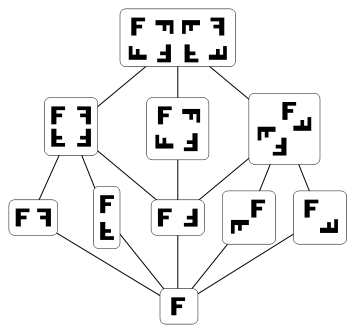
\includegraphics[height=2.1in]{D4_subgroups}
    \column{5cm} The lattice of subgroups of the dihedral group $D_4$,
    represented as groups of rotations and reflections of a plane figure. 
  \end{columns}
}


%% 9.
\frame[label=info]{
  \frametitle{...ok, but is it useful?}
  \uncover<2->{
  Lattice-theoretic information (about $\bSub[\bG]$) can be used to obtain
  group-theoretic information (about $\bG$).\\[4pt]
  \uncover<3->{
    {\bf Examples:} 
    \begin{itemize}
    \item  $\bG$ is locally cyclic if and only if $\bSub[\bG]$ is distributive.\\[4pt]
      {\O}ystein Ore, ``Structures and group theory,'' {\it Duke Math. J.} (1937)
      % Ore, ``Structures and group theory,'' {\it Duke Math. J.} (1937)
    }
    \uncover<4->{
    \item Similar lattice-theoretic characterizations exist for solvable and
      perfect groups.\\[4pt]
      Michio Suzuki, ``On the lattice of subgroups of finite groups,''\\~
      ~\phantom{MichioSuzuki}{\it Trans. AMS} (1951)\\~
      \phantom{MichioSuzuk}, ``Structure of a group and the structure of its\\
      ~\phantom{Michio Suzuki } lattice of subgroups,'' {\it Springer} (1956)
      %Suzuki, ``On the lattice of subgroups of finite groups,''\\ {\it Trans. AMS} (1951) 
    \end{itemize}
  }
}
}

% $\theta \in \Con(\bG)$ 

% \begin{frame}
%   \frametitle{Equivalence Relations}
%   \begin{itemize}
%     % \item A binary relation, $\theta \subseteq A\times A$, that is reflexive,
%     %   symmetric, and transitive is called an \emph{equivalence relation}.
%   \item Let $\Eq(A)$ be the set of equivalence relations on a set $A$.
%   \item The equivalence class of $\theta \in \Eq(A)$ containing $x$ is denoted
%     \[  x/\theta = \{y\in A | (x,y)\in \theta\}  \]
%   \item The set of all $\theta$ classes is 
%     \[  A/\theta = \{ x/\theta | x\in A\}  \]
%     and $A$ is partitioned as
%     \[  A = \bigcup \{x/\theta | x\in A\}  \]
%   \end{itemize}
% \end{frame}

%% 10.
\frame[label=eqlat]{
  \frametitle{Example: equivalence relations}
  \begin{itemize}
  \item<1->  The set of equivalence relations on a set is a 0-1 lattice:
    \[
    \bEq(A)  = \langle \Eq(A), \subseteq\rangle = \langle \Eq(A), \meet, \join\rangle
    \]
  \item<2-> $\Eq(A)\subset \power{A\times A}$ and meet is set
      intersection, while \\
      join is the equivalence generated by set union:
      % For $\alpha, \beta \in \Eq(A)$, 
      \[
      \alpha\meet \beta = \alpha \cap \beta
      \]
      \[
      % \alpha \join \beta = \bigcap \{\theta \in \Eq(A)\, \vert \, \alpha \cup \beta \subseteq \theta\}
      \alpha \join \beta = \bigcap \{\theta \in \Eq(A)\svert \alpha\leq \theta,\, \beta \leq \theta\}
      \]
    \item<3-> The greatest equivalence is the {\it all} relation:
      \[\nabla = A\times A\]
    \item<3-> The least equivalence is the {\it diagonal} relation:
      \[\Delta = \{(x,y)\in A\times A \svert x=y\} \]
    \end{itemize}
}


\frame[label=eqlatex]{
  \frametitle{Example: $\Eq(4)$}
  \begin{columns}
    \column{5cm}
    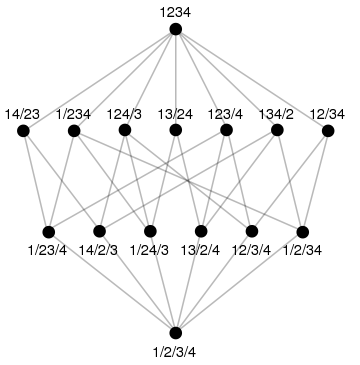
\includegraphics[height=2.1in]{Eq4}
    \column{5cm} The lattice of equivalence relations on the set of\\ four elements.
  \end{columns}
}


%%% ---- Freese frame ---- %%%

\frame[label=conglat2]{
  \frametitle{Congruence Lattices}

  \begin{itemize}
  \item
    If $f : A \to B$ is a mapping of one set to another, 
    the relation $\theta$ on $A$,% defined by 
    \[
    x \mathrel\theta y \quad \Leftrightarrow \quad f(x) = f(y)
    \]
    is an equivalence relation. 
    \item<2->
      If $\alg A$ and $\alg B$ are algebras and $f\in \Hom(\bA, \bB)$ an algebra hom,
      \[
      \theta = \ker f = \{(x,y)\in A^2  \svert f(x) = f(y)\}
      \]
      is called a \emphcyan{congruence relation} on $\alg A$.
    \item<3->
      A relation on $\alg A = \la A, F \ra$ is a congruence relation iff it is an
      equivalence relation which is a subalgebra of $\alg A^2$.
    \item<4-> The set  $\Con(\alg A)$ of congruences of $\alg A$ is a sublattice of
      $\bEq(A)$,
      \[ \bCon \alg A = \la \Con(\bA), \meet, \join \ra  \]
    \item<5->
      For groups this is the same as the lattice of normal subgroups.
    \item<6->
      For rings this is the same as the lattice of ideals.
    \item<7->
      For most classical algebras, $\bCon \alg A$ is modular.
    \item<8->
      For lattices, and the algebras of logic, $\bCon \alg A$ is distributive.
  \end{itemize}
} %end frame conglat



%\subsection{The FLRP}
%\subsection{the finite lattice representation problem}
%% 11.
\frame[label=flrp]{
  \frametitle{The finite lattice representation problem}
  \begin{definition}[representable lattice]
    Call a finite lattice \alert{representable} if it is (isomorphic to)
    the congruence lattice of a finite algebra.
  \end{definition}
  \uncover<2->{%
    \begin{block}{The $\leq$ \$1m question}
      Is every finite lattice representable?\\[6pt]
    }
    \uncover<3->{%
      Equivalently, given a finite lattice \bL, does there exist 
      a finite algebra \bA\ such that $\bCon \bA \cong \bL$?
    \end{block}
  }
  % }
}

%%%%%%%%%%%%%%  SECTION: Milestones %%%%%%%%%%%%%%%%%%%
%%  14.
\frame[label=pair]{
\frametitle{An equivalent problem in group theory}
  \begin{theorem}[\small{P\'alfy and Pudl\'ak, AU 11, 1980}]
  The following statements are equivalent:
  \begin{itemize}
  \item[(i)] Any finite lattice is isomorphic to\\
    the congruence lattice of a finite algebra.
  \item[(ii)] Any finite lattice is isomorphic to\\
    an interval in the subgroup lattice of a finite group.
  \end{itemize}
\end{theorem}
\uncover<2->{
  \begin{block}{A quote from MathSciNet reviews}{}
    {\it ``In AU 11, P\'alfy and Pudl\'ak proved that...a finite lattice is
      representable if and only if it occurs as an interval in the subgroup lattice
      of a finite group.'' }
    \\[4pt]
    \uncover<3->{
      \alert{False!} 
    }
  \end{block}
}
}
%% CONCRETE
\frame[label=concrete]{
  \frametitle{Concrete representation}
  \begin{theorem}[\small{Pudl\'ak and T\r{u}ma, AU 10, 1980}]
    A finite lattice can be embedded in $\Eq(X)$, for some finite $X$.
  \end{theorem}
\begin{itemize}
\item<2-> That is, if $\bL$ is any finite lattice, there exists a finite set $X$ with
  \[
  \bL \cong \bL'\leq \bEqX
  \]
\item<3-> Assume $\bL$ is itself \emph{concretely represented} as $\bL \leq \bEqX$
\item<4-> Define a relation $R$ on $X^X \times \Eq(X)$ as follows: 
\[
h\, R\, \theta \quad \Leftrightarrow \quad h(x) \, \theta \, h(y)
\, \text{whenever } x\, \theta\, y
\]
\item<5-> If $h\, R\, \theta$ we say ``$h$ respects $\theta$'' or
``$\theta$ admits $h$''
\end{itemize}
}

%% galois
\frame[label=galois]{
  \frametitle{YAGC}
\begin{itemize}
\item<1-> Let $\sE = \power{\Eq(X)}$ and $\sH = \power{X^X}$ be po'd by set
inclusion.
\item<2-> Define maps $\lambda: \sE \rightarrow \sH$ and $\rho: \sH \rightarrow \sE$ by
\[
\lambda(E) = \{h\in X^X \svert h\, R \,\theta \, \text{ for all } \theta\in E \} \quad (E \in \sE)
\]
\[
\rho(H) = \{\theta \in \Eq(X) \svert h\, R\, \theta \text{ for all } h\in H \} \quad (H \in \sH)
\]
\item<3-> $(\lambda, \rho)$ is a pair of
antitone maps with 
\[
\rho \lambda \geq \id_{\sE} \quad \text{ and } \quad 
\lambda \rho \geq \id_{\sH} 
\]
\item<4->$(\lambda, \rho)$ is a \emph{Galois correspondence} between $\Eq(X)$ and
  $X^X$
\item<5-> Easy consequences: \\
$\rho \lambda$ and $\lambda \rho$ are idempotent; 
$\rho\lambda\rho = \rho$ and $\lambda\rho \lambda= \lambda$;\\
$F \subseteq \rho \lambda (F)$, for any set $F \in \sE$.
\end{itemize}
}


%% CONCRETE2
\frame[label=closure]{
  \frametitle{Closure operator}
\begin{itemize}
\item The map $\rho \lambda$ is idempotent, extensive, 
and order preserving; i.e.
\[
\rho \lambda \text{ is a \emph{closure operator} on $\sE = \power{\Eq(X)}$}
\]
\item<2-> Call a set $F\in \sE$ \alert{closed} provided $\rho\lambda(F) = F$. 
%Equivalently, a set is closed if and only if it lies in $\image \rho$.
\item<3-> To reiterate, for $F\subseteq \Eq(X)$, we have
\[
F \subseteq \rho\lambda(F)\subseteq \Eq(X)
\]
and $F$ is \alert{closed} iff $\rho\lambda(F) = F$.\\[4pt]
We call $F$ \alert{dense} iff $\rho\lambda(F) = \Eq(X)$
%\item<4-> More generally, if $A$ and $B$ are subsets of $\Eq(X)$, call $A$
%  \alert{dense} in $B$ iff $\rho\lambda(A) \supseteq B$.
\item<4->If $\bL\cong \bL' \leq \bEqX$ and if $\rho\lambda(L') = \EqX$, 
then we say\\ $\bL$ can be \alert{densely embedded} in $\bEqX$.
\end{itemize}
}


\frame[label=results]{
  \frametitle{A density result}
  \begin{theorem}
    % \item<1->
    %   \underline{Problem}: Given a finite lattice $\bL$, does there exist a finite
    %   \phantom{\underline{Problem}:} algebra $\bA$ such that $\bL \cong \bCon \bA$?
    If $\bL \leq \bEqX$, then $\bL= \bCon\bA$ for some
    algebra $\mathbf{A} = \langle X, F\rangle$ if \\and only if $\bL$ is closed;
    that is, iff $\rho \lambda(L) = L$.
  \end{theorem}
%  \uncover<2->{
    \begin{itemize}
    \item<2-> 
     Much research has focused on the height two lattices $\bM_n$, 
     which are perceived as crucial for the general representation problem.
%     \begin{center}
%       \setlength{\unitlength}{1cm}
%       \begin{picture}(4,2)
%         \put(2.4,0.9){\llap{$\alg M_3$:}}
%         \put(4,0){\circle*{0.15}}
%         \put(3,1){\circle*{0.15}}
%         \put(3.3,1){\circle*{0.15}}
%         \put(3.7,1){\circle*{0.15}}
% %        \put(4,1){\circle*{0.15}}
%         \put(5,1){\circle*{0.15}}
%         \put(4,2){\circle*{0.15}}
%         \put(4,0){\line(-1,1){1}}
%         \put(4,0){\line(1,1){1}}
% %        \put(4,0){\line(0,1){1}}
%         \put(3,1){\line(1,1){1}}
% %        \put(4,1){\line(0,1){1}}
%         \put(3.3,1){\line(-1,1){1}}
%         \put(3.7,1){\line(1,1){1}}
%         \put(5,1){\line(-1,1){1}}
%       \end{picture}
%     \end{center}
%  }\uncover<3->{
 \item<3-> J.B.~Nation asked how ``bad'' can concrete representations of $\bM_3$ be in terms
   of non-closure, and do there exist ``superbad'' or dense $\bM_3$'s in $\bEq(X)$?
%  }
    \end{itemize}
 \uncover<4->{
    \begin{theorem}[\small{Snow 2009}]
      The lattice $\bEq(X)$ contains a proper dense $\bM_3$ if and only if $|X| \geq 5$.
    \end{theorem}
  }
  \uncover<5->{
    {\bf Idea of proof:} Find an $\bL \cong \bM_3$ in $\bEqX$ such that every non-trivial
    operation in $X^X$ violates some equivalence in the universe $L$ of $\bL$. 
    Then $\lambda(L)$ is trivial, so the closure $\rho \lambda (L)$ is all of $\Eq(X)$.
    John Snow proved this for $|X|$ odd.  
    %We showed the result is also true for $|X|$ even gets a bit messy, but not hard.
  }
}

\frame[label=results2]{
  \frametitle{Another density result}
  Snow's result can be generalized to $\bM_n$ as follows:\\[4pt]
  Let $\Eq(n)$ denote the set of equivalences on an $n$-element set.
  \uncover<2->{
    \begin{theorem}[{\small Snow-wjd 2009}]
      For $n\geq 1$, the lattice $\bEq(2n+1)$ contains a dense $\bM_{n+2}$.
    \end{theorem}
  }
  \uncover<3->{
    So, for any $n\geq 3$, $\bM_n$ can be densely embedded in $\bEqX$,
    for some finite set $X$. 
  }
}

\frame[label=results3]{
  \frametitle{A non-density result}
  On the other hand, we noticed that certain lattices, like $\bN_5$, are never
  densely embedded.
  \uncover<2->{
    \begin{lemma}
      Suppose $\bL = \langle L, \meet, \join\rangle$ is a complete
      $0,1$-lattice. TFAE
      \begin{enumerate}[(i)]
      \item There is an element 
        $\alpha \in L \setminus \{0_L\}$
        % $\alpha \in L$ 
        such that $\bigvee\{\gamma\in L: \gamma \ngeq \alpha \} < 1_L$
      \item There is an element $\alpha \in L \setminus \{1_L\}$ such that $\bigwedge\{\gamma\in L
        \gamma \nleq \alpha \} > 0_L$.
      \item $\bL$ is the union of a proper ideal and a proper filter.
      \end{enumerate}
      % For convenience, in the sequel we call the decomposition described in the third condition of the lemma
      % a ``nice decomposition.''
    \end{lemma}
  }
  \uncover<3->{
    \begin{theorem}[{\small wjd 2009}]
      If $\bL\ncong \mathbf{2}$ is a sublattice of $\bEqX$ satisfying
      conditions of the lemma, then $\lambda(L)$ contains a non-trivial unary function.
      % constant function that is not the identity.
    \end{theorem}
  }
  \uncover<4->{
    \begin{corollary}
      If $\bL\ncong \mathbf{2}$ is a lattice satisfying conditions of the lemma,
      then $\bL$ cannot be densely embedded in $\bEqX$.
      % and $X$ is any set, 
    \end{corollary}
  }
}

\frame[label=results4]{
  \frametitle{More non-density consequences...}
  \begin{corollary}
    If $\bL\ncong \mathbf{2}$ is a finite lattice with a prime element and $X$ is any
    set, then $\bL$ cannot be densely embedded in $\bEqX$.
  \end{corollary}
  \begin{corollary}
    If $\bL\in SD_\wedge$ is a finite semi-distributive lattice with $\bL\ncong \mathbf{2}$, 
    and $X$ is any set, then $\bL$ cannot be densely embedded in $\bEqX$.
  \end{corollary}
}

\frame[label=results5]{
  \frametitle{Finally, a closure result}
  \begin{theorem}[\small{Snow 2009}]
    Suppose $\bL \leq \bEqX$ is a closed sublattice  and $\bL'\leq \bL$ is a sublattice with universe
    $A\cup B$, where $A=\{x\in L \mid x\leq \alpha\}$ and $B=\{x\in L \mid x\leq
    \beta\}$ for some $\alpha, \beta \in L$.  Then $\bL'$ is closed.
  \end{theorem}
  \begin{itemize}
  \item<2->This is another recent result of John Snow, which he proved using \emph{primitive positive
      formulas.}
  \item<3->  An easy consequence is that all hexagons are congruence hereditary.
    That is, if a hexagon is closed, so are its sublattices.
  \end{itemize}
}



%%%%%%%%%%%%%%%%%%%%%%%%%%% SECTION: Summary %%%%%%%%%%%%%%%%%%%%%%%%%%%%%%%%%%%
%\section*{Summary}
\frame[label=summary]{
  \frametitle<presentation>{Summary}
  % Keep the summary *very short*.
  \begin{itemize}
  \item<1->
    \underline{Problem}: Given a finite lattice $\bL$, does there exist a finite\\~
    \phantom{\underline{Problem}} algebra $\bA$ such that $\bL \cong \bCon \bA$?
  \item<2-> It is generally believed the answer is no. 
  \item<3-> P\'alfy and Pudl\'ak translated it into one
    for the group theorists,\\ but still no answer...
  \item<4-> The problem can be stated very concretely in terms of partitions
    of a set allowing us to analyze many concrete examples with the computer
    and locate specific representable lattices.
  \item<5-> In recent years, the partial results have gathered significant momentum,
    and there is some hope that the full solution is forthcoming. 
  \end{itemize}
}

\frame{
\frametitle{}
\begin{center}

\includegraphics[height=2in]{thankyougreen2}
\end{center}
}
\end{document}


%%%%%%%%%%%%%%%%%%%%%%%% END DOCUMENT %%%%%%%%%%%%%%%%%%%%%%%%%%%%%%%%%%%
%%%%%%%%%%%%%%%%%%%%%%%% END DOCUMENT %%%%%%%%%%%%%%%%%%%%%%%%%%%%%%%%%%%
%%%%%%%%%%%%%%%%%%%%%%%% END DOCUMENT %%%%%%%%%%%%%%%%%%%%%%%%%%%%%%%%%%%
%%%%%%%%%%%%%%%%%%%%%%%% END DOCUMENT %%%%%%%%%%%%%%%%%%%%%%%%%%%%%%%%%%%



%% CONCRETE
\frame[label=concrete]{
  \frametitle{Concrete representation}
  \begin{theorem}[Pudl\'ak and T\r{u}ma, AU 10, 1980]
    A finite lattice can be embedded in $\Eq(X)$, for some finite $X$.
  \end{theorem}
\begin{itemize}
\item<2-> That is, if $\bL$ is any finite lattice, there exists a finite set $X$ with
  \[
  \bL \cong \bL'\leq \bEqX
  \]
\item<3-> Assume $\bL$ is itself \emph{concretely represented} as $\bL \leq \bEqX$
\item<4-> Partially order $X$ and consider the set of decreasing idempotents
\[
\idemdec = \{f\in X^X: f^2 = f \text{ and } f(x) \leq x\}.
\]
\item<5-> Partially order \idemdec\ by
\[
 f\sqsubseteq g \quad \Leftrightarrow \quad \ker f \leq \ker g.  
\]
\item<6->Then $f\sqsubseteq g$ if and only if $gf = g$, and \idemdec\ is a lattice with
\[
\idemdec \cong \bEqX
\]
\end{itemize}
}





%% 4.
\frame[label=congruences]{
  \frametitle{Congruence relations defined}
  \begin{definition}[congruence relation]
    Given $\bA = \langle A, F\rangle$, an equivalence relation $\theta\in \Eq(A)$ is\\
    a \alert{congruence} on $\bA$ if $\theta$ ``admits'' $F$ \\[4pt]
    \uncover<2->{i.e.,
      for $n$-ary $f\in F$, and elements $a_i, b_i \in A$, 
      \[
     \text{if } \; (a_i, b_i) \in \theta, \text{ then } \; 
     (f(a_1,\dots, a_n),f(b_1,\dots, b_n))\in \theta
      \]
    }
    \uncover<3->{
     or ``$f$ \emph{respects} $\theta$'' for all $f\in F$.\\[4pt] %denoted $f(\theta) \subseteq \theta$.
    }
  \uncover<4->{
    The set of all congruence relations on $\bA$ is denoted \alert{$\Con(\bA)$}.
  }
  \end{definition}
}

%% 10.
\frame[label=conglat1]{
  \frametitle{$\bCon \bA$ is a lattice}
  \begin{itemize}
    % \item  Each $\theta \in \Con(\bA)$ is a subalgebra of the product algebra.
    %   \[ \therefore \quad \Con(\bA) \subseteq \Sub[\bA\times \bA]. \]
  \item<1->  The set $\Con(\bA)$, ordered by set inclusion, is a 0-1 lattice:
    \[
    \bCon \bA  = \langle \Con(\bA), \subseteq\rangle = \langle \Con(\bA), \meet, \join\rangle
    \]
%    \vspace{-5mm}
    \begin{itemize}
    \item<2-> The greatest congruence is the {\it all} relation
      \[\nabla = A\times A\]
    \item<3-> The least congruence is the {\it diagonal} 
      \[\Delta = \{(x,y)\in A\times A \svert  x=y\} \]
    \item<4-> What are meet and join?
    \end{itemize}
  \end{itemize}
}



\frame[label=groupcong]{
  \frametitle{Examples}
  \begin{block}{What are the congruences of a group?}{
      \uncover<2->{
        For a group $\bG=\langle G, \cdot, ^{-1}, 1\rangle$,
        an equivalence $\theta\in \Eq(G)$ is\\
        a congruence on $\bG$ provided, $\forall a, b, a_i, b_i \in G$, 
        \uncover<3->{
          \[
          (a, b)\in \theta \quad \Rightarrow \quad (a^{-1}, b^{-1}) \in \theta, \;\text{ and}
          \]
        }
        \uncover<4->{
          \[
          (a_i, b_i)\in \theta \quad \Rightarrow \quad (a_1\cdot a_2, b_1\cdot b_2) \in \theta.
          \]
        }
        % $\theta \in \Con(\bG)$ 
      }
    }
  \end{block}
}





%%%%%%%%%%%%%%%%%%%%%%%  SECTION: Groups %%%%%%%%%%%%%%%%%%%%%%%%%%%%%%%%%%%
%\section{Groups}
%\subsection{G-sets}
%% 12.
\frame[label=gsets]{
  \frametitle{What is a G-set?}
  Let $\bG=\langle G, \cdot, ^{-1}, 1_G\rangle$ be a group, $A$ a set.
  \uncover<2->{
    \begin{definition}[G-set]
      A \alert{G-set} is a unary algebra $\bA= \langle A, \overline{G} \rangle$,
      where $\overline{G} = \{\bar{g}: g\in G\}$, \\[4pt]$\overline{1_G} =
      \id_A$, and  $\overline{g_1} \circ \overline{g_2} = \overline{g_1 \cdot g_2}$, for all $g_i\in G$.
    \end{definition}
  }
  \uncover<3->{%
    \begin{definition}[stabilizer]
      For any $a\in A$, the \alert{stabilizer} of $a$ is the set
      \[
      \Stab(a) = \{g\in G  \svert  \bar{g}(a) = a\}
      \]
      \phantom{x}
    \end{definition}
  }
}

\frame[label=transgsets]{
  \frametitle{G-sets: basic facts and transitivity}
%  Let $\bA = \langle A, \overline{G}\rangle$ be a G-set.
  \uncover<2->{
    \begin{block}{Basic facts about the G-set $\langle A, \overline{G}\rangle$ (efts)}{
        \begin{itemize}
        \item<2->[1.] Each $\bar{g}\in \overline{G}$ is a permutation of $A$.
        \item<3->[2.] If $[a]$ is the subalgebra generated by $a\in A$, then
          \[  
          [a] = \{ \bar{g}(a) \svert g\in G\} = \text{ the \alert{orbit} of $a$ in $A$.}
          \]
        \item<4->[3.] The stabilizer $\bStab(a)$ is a subgroup of $\bG$.
        \end{itemize}
      }
    \end{block}
  }
  \uncover<5->{
    \begin{definition}[trasitive G-set]
      If $\bA = \langle A, \overline{G}\rangle$ has only one orbit, 
      we say $\bG$ \alert{acts transitively} on $\bA$, 
      % or $\bG$ is a \alert{transitive permutation group}, 
      or $\bA$ is a \alert{transitive G-set}.
    \end{definition}
    % define stabilizer
  }
}


%\subsection{The FTTG} 
%\subsection{intervals in subgroup lattices}
%% 13.
\frame[label=fttg]{
  \frametitle{Fundamental theorem of transitive G-sets}
  % Main lemma on intervals in subgroup lattices}
  \begin{definition}[interval in a subgroup lattice]
    If \bG\ is a group and $\bH \in \Sub[\bG]$ is a subgroup, define
    \[
    [\bH, \bG] = \langle \{ \bK\in \Sub[\bG] \svert  \bH \subseteq \bK\}, \subseteq \rangle
    \]
    Call $[\bH, \bG]$ an \emph{(upper) interval} in the lattice $\bSub[G]$.
  \end{definition}
  \uncover<2->{
    \begin{theorem}
      If $\bA = \langle A, \overline{G}\rangle$ is a transitive G-set, then
      for any $a\in A$,
      \[
      \bCon \bA \cong [\bStab(a), \bG]
      \]
    \end{theorem}
  }
}

%\subsection{the seminal lemma of tct}
\frame[label=seminal]{
  \frametitle{The seminal lemma of tct}
  \begin{lemma}
      Let $\bA = \langle A, F\rangle$ be a unary algebra with 
      %$F$ a monoid, 
      $e^2=e\in F$.\\[4pt]
      Define $\bB = \langle B, G\rangle$ with
      \[
      B= e(A) \quad \text{ and } \quad G = \{ef\rvert_B : f\in F\}
      \]
      \uncover<2->{
      Then 
      \[
      \Con(\bA) \ni \theta \mapsto \theta \cap (B\times B) \in \Con(\bB)
      \]
      is a lattice epimorphism.
    }
  \end{lemma}
}

\frame[label=theorem1]{
  \frametitle{Consequence of the seminal lemma}
  \begin{theorem}
    Let $\bL$ be a finite lattice satisfying conditions (A), (B), (C).\\[4pt]
    Let $\bA = \langle A, F\rangle$ be a finite unary
    algebra of minimal cardinality such that $\bCon \bA \cong \bL$.\\[4pt]
    \uncover<2->{
      Then %(under certain conditions)
      %satisfies (A), (B), and (C), then 
      $\bA$ is a transitive G-set.
}
  \uncover<3->{
\[
\therefore \quad \bL \cong \bCon \bA \cong [\bStab(a), \bG]
\]
    }
  \end{theorem}
}







\frame[label=]{
  \frametitle{Make Titles Informative.}
\end{frame}

\section{Groups}
\subsection{G-sets}
\frame[label=gsets]{
  \frametitle{Make Titles Informative.}
\end{frame}
\subsection{Main Lemma on intervals in subgroup lattices}
\frame[label=fttg]{
  \frametitle{Make Titles Informative.}
\end{frame}

\section*{Summary}

\frame[label=]{
  \frametitle<presentation>{Summary}

  % Keep the summary *very short*.
  \begin{itemize}
  \item
    The \alert{first main message} of your talk in one or two lines.
  \item
    The \alert{second main message} of your talk in one or two lines.
  \item
    Perhaps a \alert{third message}, but not more than that.
  \end{itemize}
  
  % The following outlook is optional.
  \vskip0pt plus.5fill
  \begin{itemize}
  \item
    Outlook
    \begin{itemize}
    \item
      Something you haven't solved.
    \item
      Something else you haven't solved.
    \end{itemize}
  \end{itemize}
\end{frame}



% All of the following is optional and typically not needed. 
\appendix
\section<presentation>*{\appendixname}
\subsection<presentation>*{For Further Reading}

\frame[label=]{[allowframebreaks]
  \frametitle<presentation>{For Further Reading}
    
  \begin{thebibliography}{10}
    
  \beamertemplatebookbibitems
  % Start with overview books.

  \bibitem{Author1990}
    A.~Author.
    \newblock {\em Handbook of Everything}.
    \newblock Some Press, 1990.
 
    
  \beamertemplatearticlebibitems
  % Followed by interesting articles. Keep the list short. 

  \bibitem{Someone2000}
    S.~Someone.
    \newblock On this and that.
    \newblock {\em Journal of This and That}, 2(1):50--100,
    2000.
  \end{thebibliography}
\end{frame}

%%% \end{document}  <--- not the real end of the document!


\frame[label=]{
  \frametitle{Early Results}
  \uncover<1->{%
    \begin{block}{{\bf Theorem} (Gr\"{a}tzer and Schmidt 1963)}{}
      Every algebraic lattice is isomorphic to the congruence lattice of an algebra.
    \end{block}
  }
\note<1>{This shows that there is no lattice-theoretical condition stronger than
  algebraicity satisfied by all congruence lattices.}
\uncover<2->{%
  \begin{block}{What if the lattice is finite?}{}
  }
  \uncover<3->{%
    {\bf Problem:} Given a finite lattice \bL, does there exist a \emph{finite}
    algebra \bA\ such that $\bCon \bA \cong \bL$?
  }
  \uncover<4->{%
    \begin{itemize}
    \item status: \uncover<5->{open}
    \item age: \uncover<6->{40+ years}
    \item difficulty: \uncover<7->{\emph{what do you think?}}
    \end{itemize}
  \end{block}
}

\uncover<7->{%
  \begin{block}{{\it Representable} Lattices}{}
  }
  \uncover<8->{%
    Call a finite lattice {\bf representable} if it is the congruence lattice of a finite algebra.  
  \end{block}
}

\end{frame}



\frame[label=subgrouplattice]{
\frametitle{The Lattice $\bSub[\bG]$}
\begin{block}{}
  The {\it subgroup lattice} of a group \bG\ is denoted
\[
\bSub[\bG] = \langle \Sub[\bG], \subseteq \rangle = \langle \Sub[\bG],\meet, \join\rangle 
\]
The elements are the subgroups of \bG, partially ordered by set inclusion.
\end{block}

\begin{block}{}
For subgroups $H, K \leq G$, 
\begin{itemize}
\item The meet is intersection: 
\[
H\meet K = H\cap K
\]
\item The join is the subgroup generated by the union:
\[
H\join K = \bigcap \{J\leq G \svert  H\cup K \subseteq J\}
\]
\end{itemize}  
\end{block}
}


% Structuring a talk is a difficult task and the following structure
% may not be suitable. Here are some rules that apply for this
% solution: 

% - Exactly two or three sections (other than the summary).
% - At *most* three subsections per section.
% - Talk about 30s to 2min per frame. So there should be between about
%   15 and 30 frames, all told.

% - A conference audience is likely to know very little of what you
%   are going to talk about. So *simplify*!
% - In a 20min talk, getting the main ideas across is hard
%   enough. Leave out details, even if it means being less precise than
%   you think necessary.
% - If you omit details that are vital to the proof/implementation,
%   just say so once. Everybody will be happy with that.

%     {\it Example:} $\bSub(V)$, the subspaces of a vector space.

% \frame[label=]{
%   \frametitle{Some History...}
%   \begin{itemize}
%   \item[pjm 82] {\bf Theorem (Freese, Lampe, Taylor 1979)} If $V$ is an infinite vector space
%     over an uncountable field $F$, then $\bCon(\bA)\cong \bSub(V)$ implies $\bA$ has at least $|F|$ operations.\\[4pt]
% %    {\it Key point:} As $V$ is infinite, the largest element or ``unit'' of $\bSub(V)$ is not
% %    compact. The next result shows that a compact unit is essential.
%   \item[pjm 103] {\bf Theorem (Lampe 1982)} Every algebraic lattice with compact unit is
%     isomorphic to the congruence lattice of some groupoid. 
%   \end{itemize}
% \end{frame}
% % Ji\v{r}\'i 
% %P\'eter 



\frame[label=conglat2]{
  \frametitle{The Lattice of Congruence Relations}
  \begin{itemize}
  \item $\bCon \bA$ is a complete lattice.
  \item The \emph{compact} elements of $\bCon \bA$ are the finitely generated congruences.
  \item $\bCon \bA$ is an \emph{algebraic} lattice.
  \end{itemize}
Conversely, Gr\"{a}tzer and Schmidt (1962) proved that any algebraic lattice is a
congruence lattice.
  \begin{itemize}
  \item 
  \end{itemize}
  Again there is a converse: By a theorem of , every algebraic lattice is isomorphic to Con(A) for some algebra A.





  \uncover<3->{%
    \begin{definition}[arity]
      The \alert{arity} of an operation $f \in F$ is the number of operands.
      \begin{itemize}
      \item<4-> $f$ is $n$-\emph{ary} if it maps $A^n$ into $A$
      \item<5-> \emph{nullary}, \emph{unary}, \emph{binary}, and \emph{ternary} 
        operations have arities 0, 1, 2, and 3, respectively
      \end{itemize}
    \end{definition}
















%% 2.
\frame[label=background]{
  \frametitle{Background}
  \begin{columns}
    \column{70mm}
%    \begin{theorem}[Gr\"{a}tzer-Schmidt, Acta Szeged 24, 1963]
    \begin{theorem}[Gr\"{a}tzer-Schmidt, 1963]
      Every algebraic lattice is isomorphic to\\
      the congruence lattice of an algebra.
    \end{theorem}
 %   \column{4cm}
  \end{columns}
%  \note<1>{This shows that there is no lattice-theoretical condition stronger than
%    algebraicity satisfied by all congruence lattices.}
  \uncover<2->{%
  \begin{columns}
%    \column{3cm}
    \column{85mm}
    \begin{block}{What if the lattice is finite?}{}
    }
    \uncover<3->{%
      \underline{Problem}: Given a finite lattice \bL, does there exist
      \phantom{\underline{Problem}:} a \emph{finite} algebra \bA\ such that $\bCon\bA \cong \bL$?
    }
    \uncover<4->{%
  \begin{columns}
    \column{17mm}
    \column{85mm}
      \begin{itemize}
      \item[\underline{status}:] open
      \item[\underline{age}:] 45+ years
%      \item[\underline{difficulty}:] probably hard
      \end{itemize}
    \end{columns}
    \end{block}
  \end{columns}
  }
}% end frame "early"





%% 1.
% \frame[label=lattices]{
%   \frametitle{What is a Lattice?}
%   \uncover<2->{%
%     \begin{definition}
%       A \alert{lattice} is a partially ordered set in which every pair of elements has
%       a g.l.b.~and a l.u.b.
%     \end{definition}
%   }

%   \uncover<3->{%
%     \begin{examples}
%       \begin{itemize}
%       \item Subsets of a set
%       \item Closed subsets of a topology.
%       \item Subgroups of a group.
%       \end{itemize}
%     \end{examples}
%   }
% } % end frame lattices





\frame[label=algexamples]{
  \frametitle{Examples}
  \begin{definition}%[group]
    A \alert{group} is an algebra $\bG = \langle G, \cdot, ^{-1}, 1\rangle$ 
    with binary, unary, and nullary operations satisfying, $\forall x, y, z\in G$,
    \begin{itemize}
    \item[G1:] $x\cdot (y\cdot z) \approx (x\cdot y)\cdot z$
    \item[G2:] $x\cdot 1\approx 1\cdot x \approx x$
    \item[G3:] $x\cdot x^{-1} \approx x^{-1}\cdot x \approx1$
%     \item[G1:] $x\cdot (y\cdot z) \approx (x\cdot y)\cdot z$
%     \item[G2:] $x\cdot 1\approx 1\cdot x \approx x$
%     \item[G3:] $x\cdot x^{-1} \approx x^{-1}\cdot x \approx 1$
    \end{itemize}
  \end{definition}
  \uncover<2->{%
    \begin{definition}
      A \alert{lattice} is an algebra $\bL = \langle L, \meet, \join\rangle$ with
      universe $L$, a partially ordered set, and binary operations:
      \begin{itemize}
      \item<2->[] $x\meet y = \text{g.l.b.}(x,y)$ \phantom{x} the ``meet'' of $x$ and $y$
      \item<2->[] $x\join y = \text{l.u.b.}(x,y)$ \phantom{x} the ``join'' of $x$ and $y$
      \end{itemize}
    \end{definition}
  }
  \uncover<3->{%
    \begin{itemize}
     \item Examples: subsets of a set, closed subsets of a topology,
       subgroups of a group, normal subgroups of a group,
ideals of a ring, submodules of a module,
invariant subspaces of an operator, etc.
%     \item Examples: subsets of a set, closed subsets of a topology,
%       \phantom{Examples: }subgroups of a group, normal subgroups of a group,\\
%       \phantom{Examples: }ideals of a ring, submodules of a module, \\
%       \phantom{Examples: }invariant subspaces of an operator, etc.
    \end{itemize}
  }
}
